 
\chapter{Problema SHE como un problema de control óptimo}


Abordaremos el problema de \emph{SHE} de simetría de media onda y de dos niveles. Suponiendo la simetría de media onda de una onda $f(\omega t)$ se puede descomponer en serie de Fourier:

\begin{equation}
    f(\omega t) = \sum_{n=1}^{\infty} \Bigg[ a_n \sin((2n-1)\omega t) + b_n cos((2n-1)\omega t)\Bigg]
\end{equation}

donde:

\begin{equation}
    a_n = \frac{2}{\pi} \int_0^\pi f(\omega t) \sin((2m-1) \omega t) d(\omega t) 
\end{equation}

\begin{equation}
    b_n = \frac{2}{\pi} \int_0^\pi f(\omega t) \cos((2m-1) \omega t) d(\omega t) 
\end{equation}

Para simplificar harémos el cambio de variable $\tau = \omega t$. Entonces las expresiones anteriores se pueden escribir de la siguiente forma:

\begin{equation}
    f(\tau) = \sum_{n=1}^{\infty} \Bigg[ a_n \sin((2n-1)\tau) + b_n cos((2n-1)\tau)\Bigg]
\end{equation}

\begin{equation}\label{an}
    a_n = \frac{2}{\pi} \int_0^\pi f(\tau) \sin((2m-1) \tau) d\tau 
\end{equation}
\begin{equation}\label{bn}
    b_n = \frac{2}{\pi} \int_0^\pi f(\tau) \cos((2m-1) \tau) d\tau 
\end{equation}

Deberemos notar que las expresiones (\ref{an}) y (\ref{bn}) pueden ser escritas en forma de ecuación diferencial:

\begin{gather}
    a_n = \frac{2}{\pi} \int_0^\pi f(\tau) \sin((2m-1) \tau) d\tau  \  \Rightarrow \ \frac{d \alpha_n}{d\tau} = \frac{2}{\pi}f(\tau) \sin((2m-1)\tau) \ | \ \alpha_n(0) = 0\\ 
    b_n = \frac{2}{\pi} \int_0^\pi f(\tau) \cos((2m-1) \tau) d\tau  \  \Rightarrow \ \frac{d \beta_n}{d\tau} = \frac{2}{\pi}f(\tau) \cos((2m-1)\tau) \ | \ \beta_n(0) = 0
\end{gather}

Entonces dado una función $f(\tau)$ podemos obtener los coeficiente de Fourier $a_n$ y $b_n$ resolviendo el siguiente sistema de ecuaciones diferenciales hasta tiempo $\tau=\pi$.

\begin{gather}
    \frac{d \alpha_n}{d\tau} = \frac{2}{\pi}f(\tau) \sin((2m-1)\tau) \ | \ \alpha_n(0) = 0 \\
    \frac{d \beta_n}{d\tau} = \frac{2}{\pi}f(\tau) \cos((2m-1)\tau) \ | \ \beta_n(0) = 0
\end{gather}

\section{Problema de control óptimo para SHE}
De esta forma si tenemos un vector de objetivo $\bm{a}_T = [a_1^T,a_2^T,\dots,a_{M}^T] \in \mathbb{R}^M$ y  $\bm{b}_T = [b_1^T,b_2^T,\dots,b_{M}^T] \in \mathbb{R}^M$, donde $M$ es el número de armónicos impares de interés, podemos plantear el siguiente problema de control óptimo:

\begin{gather}
    \min_{f(\tau) \in \mathcal{F}} \big[  || \bm{\alpha}(T) - \bm{a}_T ||^2  + || \bm{\beta}(T) - \bm{b}_T ||^2 \big] \\
    \text{sujeto a: }
    \begin{cases}
        \frac{d \alpha_n}{d\tau} = \frac{2}{\pi}  f(\tau) \sin[(2m-1) \tau ] \ \ \ | \ \ \ a(0) = 0   \\
        \frac{d \beta_n}{d\tau}  = \frac{2}{\pi}  f(\tau) \cos[(2m-1) \tau ] \ \ \ | \ \ \ b(0) = 0   \\
    \end{cases}
    \forall n \in \{ 1, \dots,M\}  \\ 
    \text{sujeto a: } f_{min} < f(\tau) < f_{max} \ | \ \forall \ \tau \in (0,\pi)  
\end{gather}

Con tiempo final $T = \pi$


\section{Condiciones de optimalidad  para el problem de control óptimo para SHE}


Siguiendo el principio de mínimo de Pontryagin construiremos el Hamiltoniano:

\begin{gather}
    H = \sum_{m=1}^M \Bigg[ p_\alpha^m \Bigg(\frac{2}{\pi} f(\tau) \sin((2m-1)\tau)\Bigg) + p_\beta^m \Bigg(\frac{2}{\pi} f(\tau) \cos((2m-1)\tau)\Bigg) \Bigg] \\
    H = \frac{2}{\pi} f(\tau)\sum_{m=1}^M \Bigg[  p_\alpha^m   \sin \big[(2m-1)\tau)\big] 
                                                + p_\beta^m   \cos \big[ (2m-1)\tau)\big] \Bigg]
\end{gather}
 
La ecuación de adjunto se puede calcular de la siguiente manera:

\begin{gather}
    \frac{d p_\alpha^m}{d \tau} = \frac{\partial H }{\partial \alpha_m} = 0 \ \ \text{y} \ \    \frac{d p_\beta^m}{d \tau} = \frac{\partial H }{\partial \beta_m} = 0  
\end{gather}

Es decir la componente $p_\alpha^n$ y $p_\beta^n$ son constantes.
\newline

Si llamamos $\Psi(\bm{\alpha},\bm{\beta})$ a:

\begin{gather}
    \Psi(\bm{\alpha},\bm{\beta}) = \big[  || \bm{\alpha}(T) - \bm{a}_T ||^2  + || \bm{\beta}(T) - \bm{b}_T ||^2 \big]
\end{gather}
Utilizando la condición final del adjunto:

\begin{gather}
    p_\alpha^m(T) = \frac{d\Psi}{d\alpha_m} = 2(\bm{\alpha_m(T) - \bm{a}^T_n})\\
    p_\beta^m(T) = \frac{d\Psi}{d\beta_m} = 2(\bm{\beta_m(T) - \bm{b}^T_n})
\end{gather}


Si llamamos $G(\tau,\bm{p}_\alpha,\bm{p}_\beta)$ a:

\begin{gather}
    G(\tau,\bm{p}_\alpha,\bm{p}_\beta) =  \frac{2}{\pi}\sum_{m=1}^M \Bigg[  p_\alpha^m   \sin \big[(2m-1)\tau)\big] 
    + p_\beta^m   \cos \big[ (2m-1)\tau)\big] \Bigg]
\end{gather}

Entonces el Hamiltoniano se puede escribir como: 

\begin{gather}
    H = G(\tau,\bm{p}_\alpha,\bm{p}_\beta) f(\tau)
\end{gather}

Aplicando el principio del mínimo de Pontryagin podemo hallar la forma de $f^*$ 

\begin{gather}
    \min_{f \in \mathcal{F}} H \rightarrow f^* = \begin{cases}
        f_{min} \ \  \text{si} \ \ G(\tau,\bm{p}_\alpha,\bm{p}_\beta) > 0  \\
        f_{max} \ \ \text{si}  \ \ G(\tau,\bm{p}_\alpha,\bm{p}_\beta) < 0  
    \end{cases}
\end{gather}

Obtenemos un control \emph{Bang-Bang}, es decir una función que toma solo dos valores (\ref{figbang})



\begin{figure}[]
    \centering
    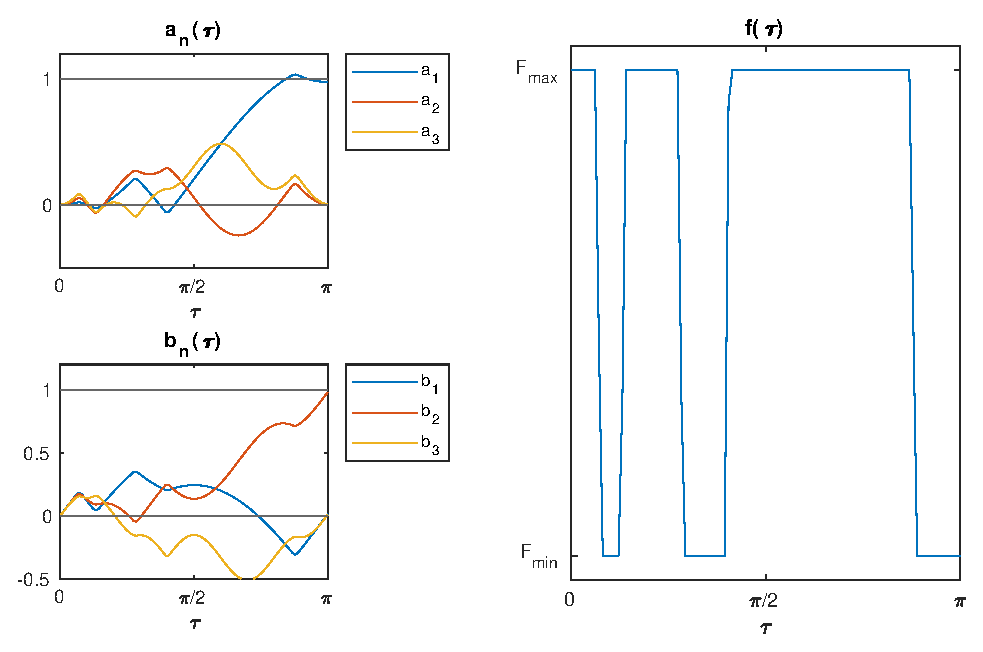
\includegraphics[scale=0.7]{fig/img03.eps}
    \caption{Solución numérico del problema de control óptimo. $a_T = [1 \ 0 \ 0 \ 0]^T$ y 
    $b_T = [1 \ 0 \ 1 \ 0]^T$}
    \label{figbang}
\end{figure}

\end{document}

